%ssssFile: paper.tex
%ss Created: Sat Dec 06 04:00 PM 2014 E
%
\documentclass[letterpaper,12pt]{article}
% Change the header if you're going to change this.
 
% Possible packages - uncomment to use
\usepackage{amsmath} % Needed for math stuff
%\usepackage{lastpage}sss% Finds last page
\usepackage{amssymb} % Needed for some math symbols
\usepackage{graphicx}% Needed for graphics
\usepackage[usenames,dvipsnames]{xcolor} % Needed for graphics and color
%\usepackage{setspace}sss% Needed to set single/double spacing
\usepackage{float} % Better placement of figures & tables
\usepackage{hyperref} % Can have actual links
\usepackage{mathpazo}
\usepackage[linesnumbered,vlined,ruled]{algorithm2e} % algorithm

%Suggested by TeXworks
\usepackage[utf8]{inputenc} % set input encoding (not needed with XeLaTeX)
\usepackage{verbatim} % lets you do verbatim text
 
% Sets the page margins to 1 inch each side
\usepackage[margin=1in]{geometry}
\geometry{letterpaper}
%\addtolength{\oddsidemargin}{-0.875in} 
%\addtolength{\evensidemargin}{-0.875in} 
%\addtolength{\textwidth}{1.75in} 
%\addtolength{\topmargin}{-.875in} 
%\addtolength{\textheight}{1.75in}

\frenchspacing

% Uncomment this section if you wish to have a header.
\usepackage{fancyhdr} 
\pagestyle{fancy} 
\renewcommand{\headrulewidth}{0.5pt} % customize the layout... 
\lhead{Chen, W., Sim, B., Shi, A.} \chead{Applied Math 205 Final Project} 
\rhead{Fall 2014} 
\lfoot{} \cfoot{\thepage} \rfoot{}


\begin{document}
\title{Explorations to Optimize the Parareal Algorithm \\to Solve ODEs in Given Applications}
\author{Wesley Chen, Brandon Sim, Andy Shi \\
Harvard University, Applied Math 205 Final Project}
\date{December 10, 2014}

% No indentation for new paragraphs
\setlength\parindent{0pt}

% Space between each new paragraph
\setlength\parskip{2ex}

% Put your stuff here
%\twocolumn[
%\begin{@twocolumnfalse}
\maketitle
\begin{abstract}

We look to achieve strong scaling in parallelizing numerical ODE methods. We test both parallelism by result space as well as parallelism by time, with the Parareal algorithm, to solve various ODEs.  We measure performance and compare in
terms of accuracy, speedup and efficiency. We provide some theoretical analysis for the Parareal algorithm and compare its tradeoff to paralleism by space, For the Parareal agorithm, we observe
light speedups in our small scale tests up to 64 processors on Harvard's
Odyssey cluster. We analyze possible reasons as to why our implementation
may not be ideal and some tradeoffs that are taken in the Parareal
implementation. Further optimizations are proposed and rationalized as next
steps including ports of to C++ using BLAS. Our code is written in python using mpi4py. We compare tests from various data sources from basic exponential ODEs to larger grids of ODEs to solve for in applications like diffusion and sound wave propagation.

\end{abstract}
%\end{@twocolumnfalse}
%]

\clearpage

\tableofcontents

\clearpage

\section{Background}

\subsection{Numerical Methods and Parallelization}
Solving systems of differential equations can be a computationally expensive
task. The error of most algorithms scales on the stepsize of the discretization
of time. However, stepsize in time is also proportional to the computation
required. It would be nice to allow for strong scaling where a problem can be
solved in a reasonable time for very small time steps.

Another obstacle to trying to parallelize numerical methods is that the methods
are inherently serial in time---in that evaluation of the next time point $n+1$
depends on the previous values, say those at time $n-1$ and $n$. This setup
does not allow for parallelism. The only way to incorporate parallelism is to
create schemes that have parallelizable components---such as an update or a
refinement built on top of a more basic method first computed in serial. As will be discussed and analyzed in the
metodology section, one such scheme would be the parareal algorithm. As an
overview, the parareal algorithm first does a coarse (low-order and fast)
approximation, then seeks to iteratively correct using smaller, more refined
numerical methods done in parallel from approximated starting points
approximated by the coarse solution.

An alternative paradigm to applying parallelism to numerical methods is the
parallelism by space paradigm, where the result vector space is divided up to
different regions and sent to different responsible processors. In this way,
each processor sees a similar but smaller-scale problem---weak scaling. This
method is expected to outperform the parallel in time paradigm simply because
the task is embarassingly parallel, being able to be naturally divided
into smaller but identical in method problems. There is no serial component in
this algorithm and should be exhibit both strong and weak scaling.

In general, the division in space paradigm is more intuitive to parallelize and
will often lead to greater speedups because there is no serial component. The main tradeoff however, is that knowing how to divide the resultant system requires knowledge of problem-specific details. Thus, this approach lacks the
general stability and theoretical proofs (of error and convergence) that schemes which parallelize in
time can offer.

\subsection{Measuring Parallel Performance}

\section{Methodology}

The parareal algorithm, developed by Lions, Maday and Turinici in 2001, CITE is
a generalalized algorithm which allows for parallelization in time. It does so by using a
cheaper ($g_{\Delta t}$)---lower order or lesser resolution, approximation first which it then corrects by evaluating segments with a finer method ($g_{fine}$). The correction step from the approximation can be done in parallel. Multiple iterations can be performed to achieve an error provably asymptotically equal to a full serial computation of $g_{fine}$. The exact number of iterations required to achieve certain levels of convergence depends on the problem and must be tuned top optimize for speedup for a given system. In summary, the algorithm is $k$ repetitions of a
correction process which requires running updated by a finer method run in parallel for subsections.

\begin{algorithm}[t]
    \KwIn{Temporal discretization $t_n = t_0 + n \Delta t, \, n = 1,2,\ldots,N$}
    \KwIn{Coarse scheme $g_{\Delta t}$}
    \KwIn{Finersscheme $g_{\textnormal{fine}}$}
    Compute $u^1_{n+1} = g_{\Delta t}(t_n, u^1_n)$\;
    Compute the corrections $\delta g_n(u^1_n) = g_{\textnormal{fine}}(t_n,
    u^1_n) - g_{\Delta t}(t_n, u^1_n)$ in parallel\;
    Add the prediction and correction terms as $u^2_{n+1} = g_{\Delta t}(t_n,
    u^2_n) + \delta g_n(u^1_n)$\;
    Repeat steps 2 and 3, incrementing the iteration label and using $u^{k+1}_0
    = u^1_0$ as the initial condition\;
 \caption{Parareal}
 \label{alg:parareal}
\end{algorithm}

The beauty is the parareal method can be adapted into many different versions with different choices of the $g_{\Delta t}$ and $g_{fine}$ solution operators.  The $g_{fine}$ solution is to a more computationally expensive method but assumed to provide either greater resolution or lower error.  Most of the time this will be a higher order method, but can also be a greater sampling of the same order method used in the coarse version.  The exact optimum pairing is problem-specific and the code is written so that a different "n-order method step" function could be written and then replaced into the code.

\subsection{Visualization of Scheme}

bksim TODO put a graph because maybe it'll help? the slides have a version

\subsection{Stability of the Parareal}

With the Parareal method, it is possible to combine ODE solvers. The stability region depends on both $g_{\Delta t}$ and $g_{\textnormal{fine}}$, and the
equation being solved. 

FROM THE SLIDES 

TODO BKSIM? ASHI carry?

\subsection{Convergence of the Parareal}

TODO BKSIM

Assume the coarse operator $g_{\Delta t}$ is order $m$ and is Lipshitz, and the
fine solution operator $g_{\textnormal{fine}}$ is a sufficiently accurate
approximation to the analytic operator so we may replace $g_{\textnormal{fine}}
\to g$. 

\emph{Theorem}: The order of accuracy of the Parareal method with coarse
solution operator $g_{\Delta t}$ and fine operator $g$ is $mk$. Can be proved by
induction. 

SHALL WE DO IT THEN?

\subsection{Error of the Parareal}

FROM THE SLIDES? + Adjust?
TODO BKSIM? ASHI carry?

Show that this parareal method will approach, with large enough $k$ (enough
iterations) to approach the error of the fine method. However, with too large of
a $k$ and a lower quality factor (ratio of fine to coarse), the time for the
parareal could potentially take longer than the direct serial computation.

\subsection{Parallel Tradeoff Analysis}

ashi TODO

Let's say the coarse operator runs in time $t$, and the fine operator runs in
time $Q \cdot t$. Assume we have $N$ processors and we perform $k$ correction
steps. Then, the runtime of Parareal is, assuming negligible setup and
aggregation time,

\begin{equation}
t + k(t + \frac{Qt}{N}).
\end{equation}

The first t seconds comes from the first coarse approximation, without which the parareal algorithm degenerates to $g_{\Delta t}$,  In order for there to be a speedup relative to the fine operator, we require
that $t + k(t + Qt/N) < Qt$, or $k < \frac{Q - 1}{1 + Q/N}$ or $N > \frac{Qk}{Q
- 1 - k}$. This can be tuned with by either adjusting the the quality factor or reducing the number of iterations, but the number of iterations, k, is important for error convergence to that of $g_{fine}$.  However, this optimal k is a problem-specific parameter and must be optimized for.


\subsection{Explored Tests}

We wished to explore certain tests that would span the space of possible
parameters to the parareal as well as possible applications in different ODE
systems. Because there were so many different versions and parameteres for the parareal to test,

\section{Results and Discussion}

\subsection{Comparison to Serial with $g_{fine}$ as a Forward Euler with
Smaller $\Delta t$}

We implemented the Parareal algorithm in Python, using mpi4py to parallelize it.
Our coarse operator was forward Euler step, with 100 steps, while the fine
operator was forward Euler, with $Q * 100$ steps, where $Q$ is the quality
factor. We tested the Parareal algorithm on two sets of differential equations:

\[
y'(t) = f(t, y) = \lambda y, \, y(0) = 1
\]
\[
y''(t) + 2y'(t) + 5y(t) = 0, \, y(0) = 1 \, y'(0) = 0.
\]

We ran the algorithm on different numbers of processors and varied $k$ and $Q$. 

Varying Iterations:

Varying Quality Factor:
We define the quality factor in this case for how many times smaller the Euler method used for $g_{fine}$ is compared to the Euler method used for $g_{\Delta t}$

Changing the ODE

TODO ashi sort out the figure and match and replace if needbe

\begin{figure}
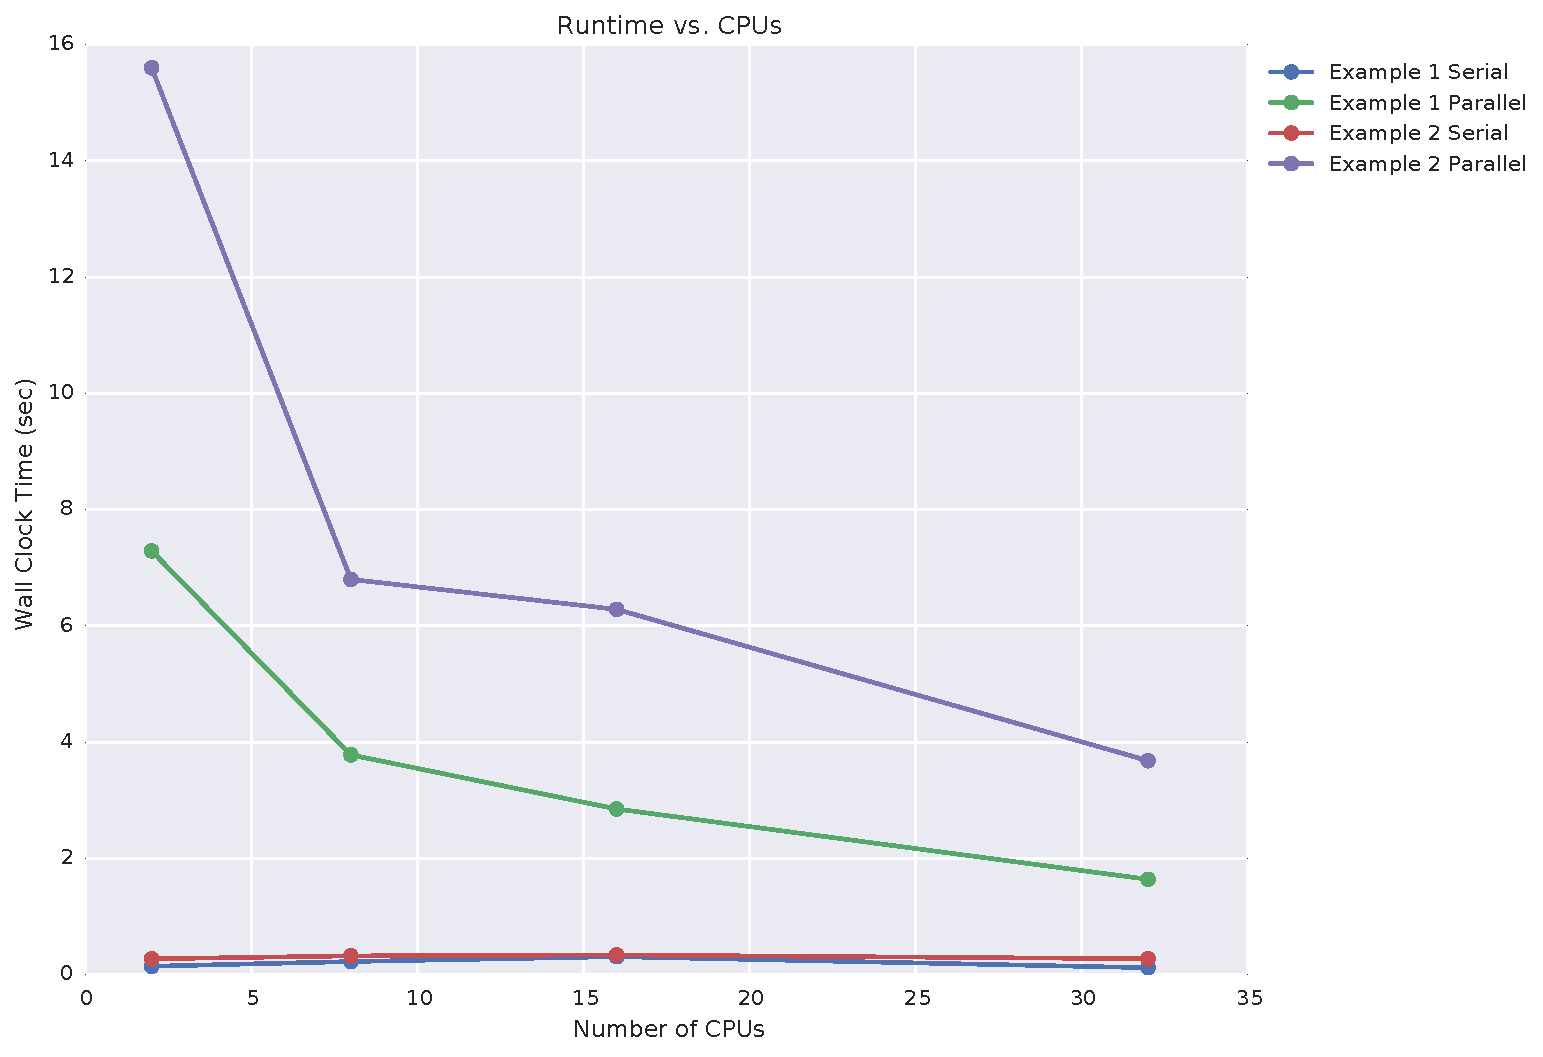
\includegraphics[width=0.75\textwidth]{data/runtime_vs_cpus.pdf}
\caption{Running time vs. number of CPUs.}
\label{fig:run_v_cpu}
\end{figure}

\begin{figure}
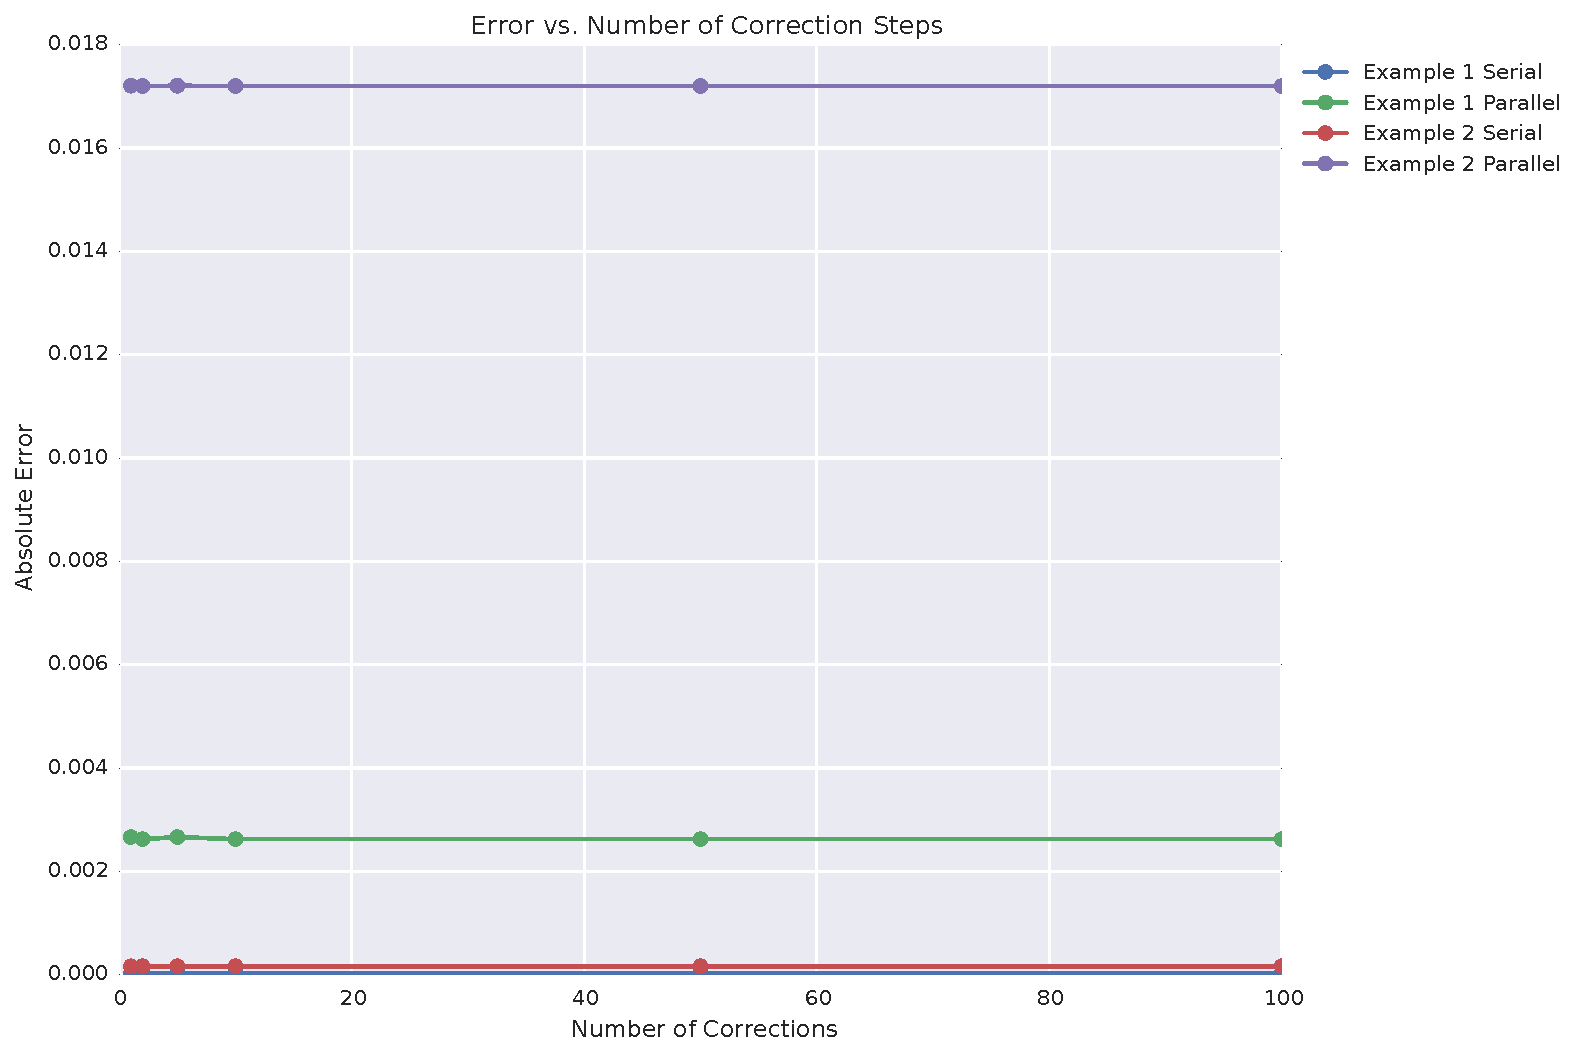
\includegraphics[width=0.75\linewidth]{data/error_vs_corrections.pdf}
\caption{Error vs. number of correction steps.}
\label{fig:err_v_k}
\end{figure}

\begin{figure}
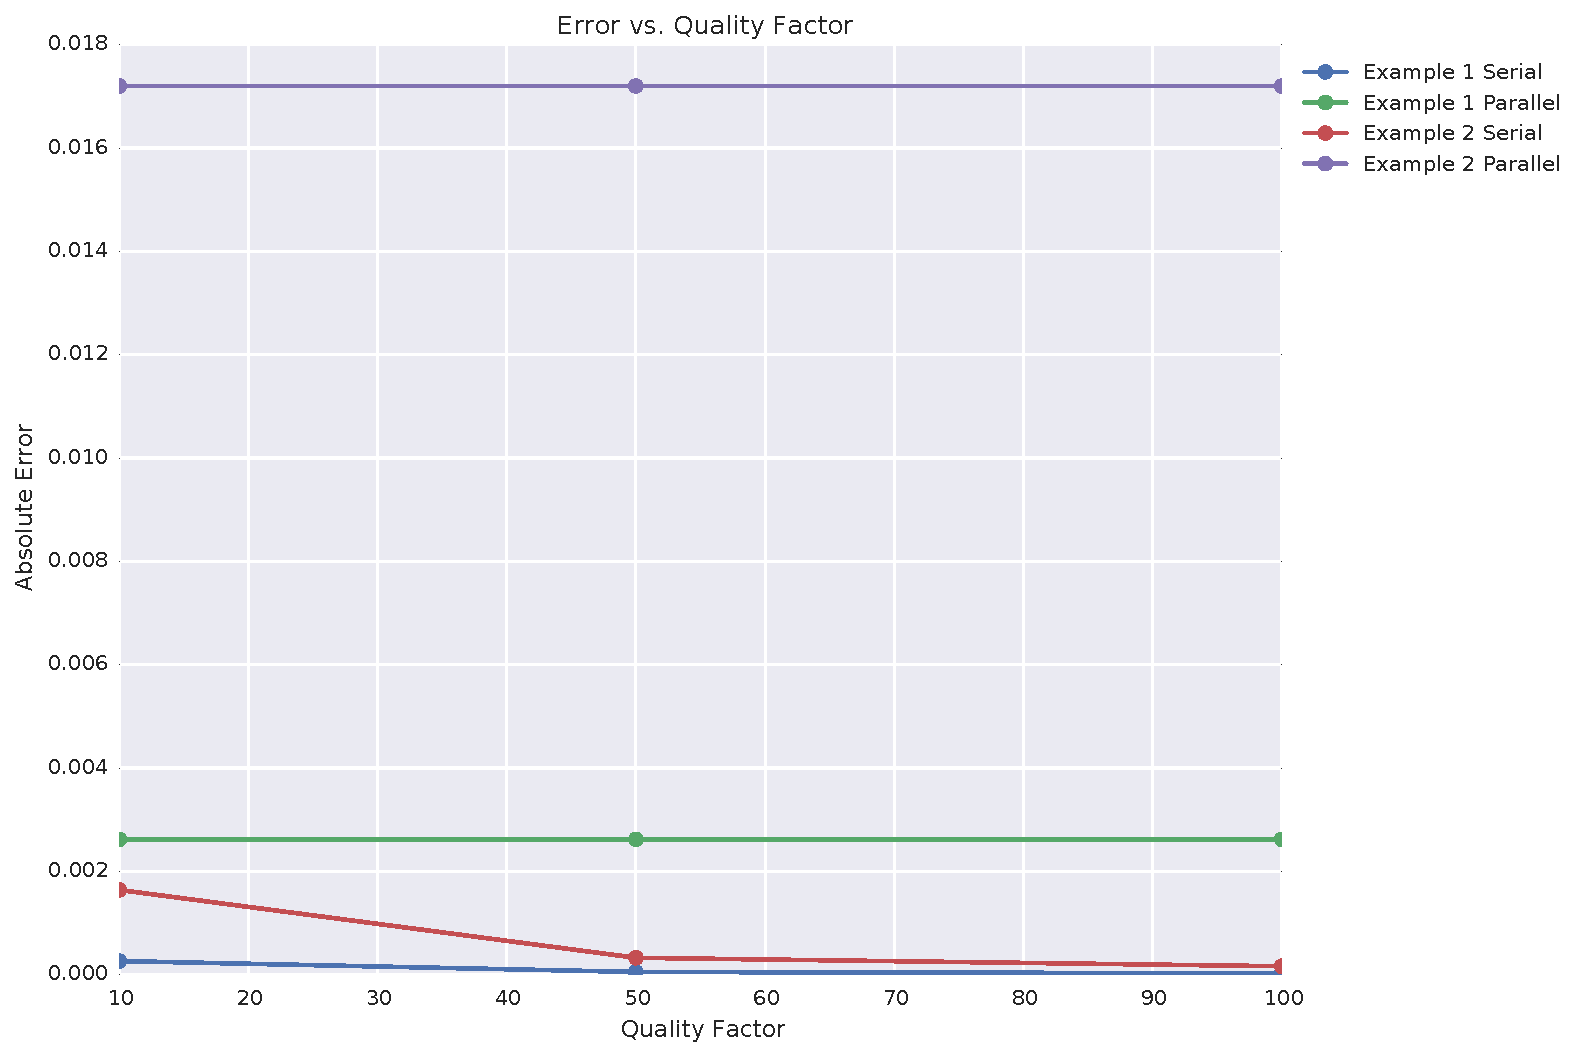
\includegraphics[width=0.75\linewidth]{data/error_vs_qualityfactor.pdf}
\caption{Error vs. quality factor of the fine operator}
\label{fig:err_v_q}
\end{figure}

\begin{figure}
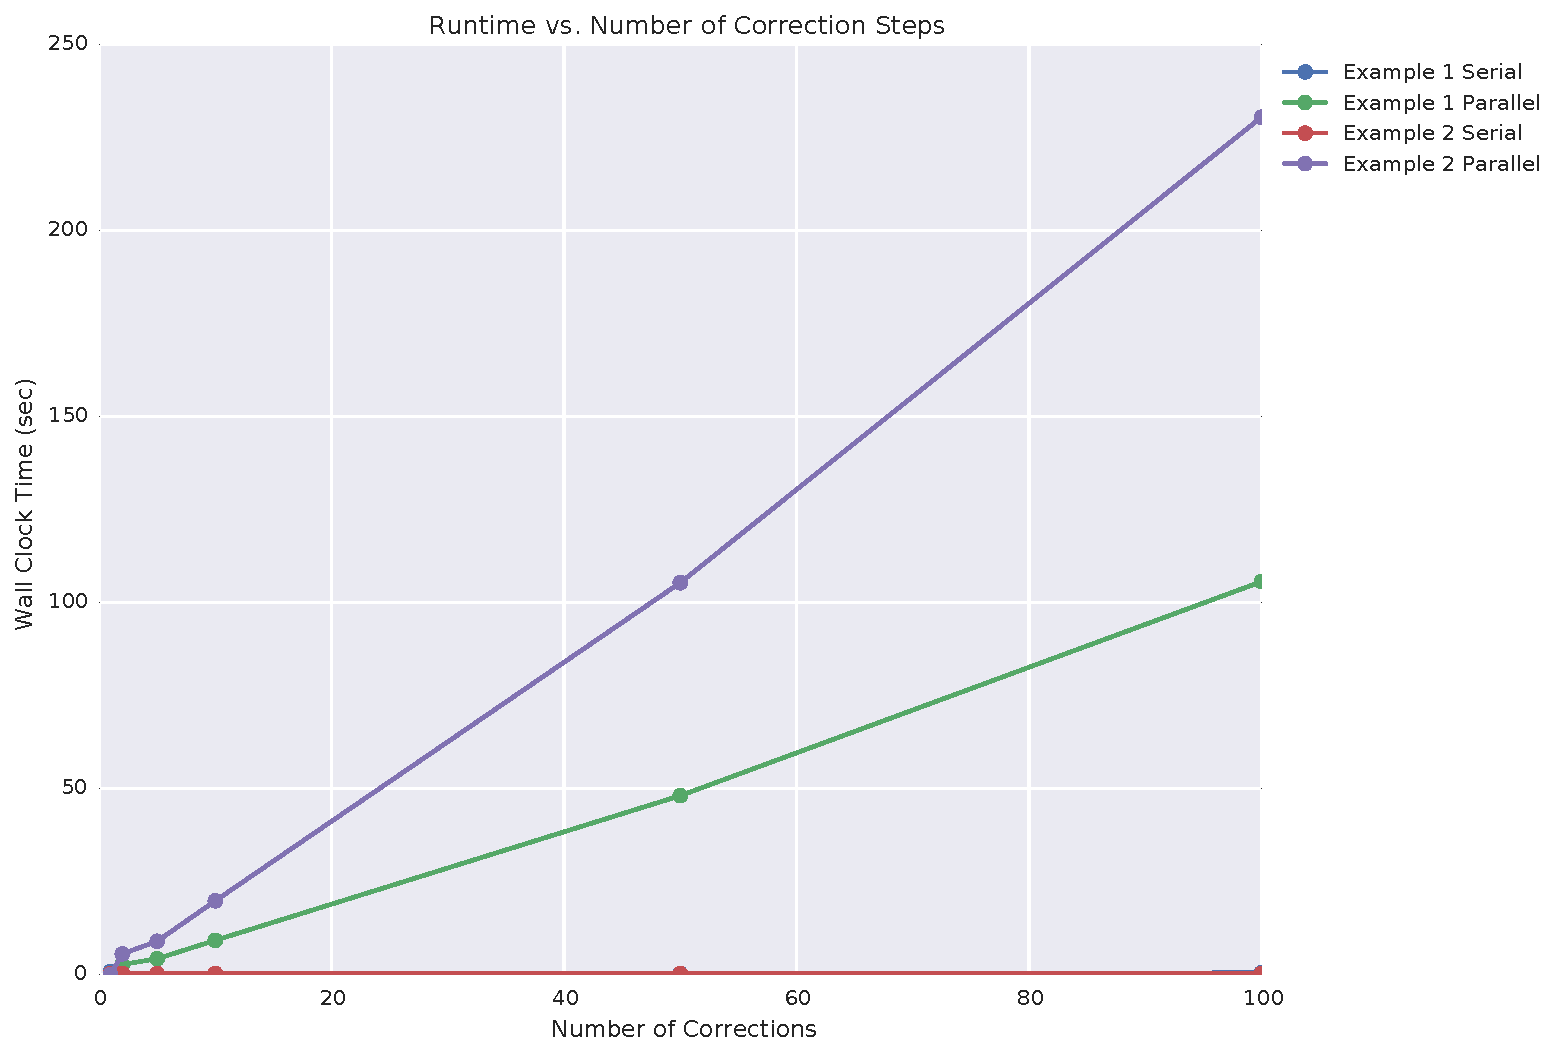
\includegraphics[width=0.75\linewidth]{data/runtime_vs_corrections.pdf}
\caption{Running time as a function of the number of correction steps.}
\label{fig:run_v_k}
\end{figure}

\subsection{Comparison to Serial with $g_{fine}$ as Higher Order Methods}

TODO team

IDEALLY WE SHOW THE SAME GRAPHS AS THE ABOVE WITH ALL THE VARIATIONS TESTED

\subsection{Parallelism by Space Paradigm}

For the speaker problem, we designed a problem-specific method to parallelize in space and divide Pierce Hall into subsections such that each processor would receive a division of the building to compute. We wish to strong scaling, in which the computation time of our parallel method will decrease as we increase the number of processors. We compare this version to the serial version we did for Homework 4.

bksim TODO GET DATA, AS REQUIRED FROM ABOVE, SHOW GRAPHS

\subsection{Parallelism Paradigm Comparisons}

Now with 3 different parallel implementations, two in time wiht the parareal, one in space,  we compare across TODO WESLSEY

TODO compare the computation times (and perhaps a slight change in accuracy of the results) between both parareal methods the best in the sections before hand

TODO bsim and ashi show graphs and some times for the forward Euler parareal
versions---the fastest ones or both if we have both implemented

\subsection{Comparison to C++ Implementations}

The numpy environment combined with the required structure of MPI required
certain type/data structure conversions which will take time.not not cunot cu

\subsection{Summary of Performance}

TODO team

\subsection{Strong and Weak Scaling Analysis}

ashi TODO by taking some numbers and following
\url{https://www.sharcnet.ca/help/index.php/Measuring_Parallel_Scaling_Performance}

\subsection{Demonstrating Scaling}

As we can see, we do see the effects of strong scaling

TODO analyze

\subsection{Possible Optimizations}

TODO WESLEY

\section{Conclusion and Future Work}

We see that (HOPE IT WORKS WELL OR ELSE...) Most of the further work would be in
optimization. We are trying to measure performance in Python, which is not the
ideal benchmarking language for efficiency and speedups. A port over to C++
using the MPI libraries in C++ rather than the mpi4py libraries in python would
be ideal. Other optimizations mentioned above could also be implemented. To
further explore the parareal algorithm would involve many test cases and to see
how the parareal algorithm compares to other approaches---since the actual time
and iterations necessary depend on the system of ODEs to solve.

On the other hand, parallelism by space already requires a very problem-specific
design. The strong scaling efficiency of parallelism by space is high and is
conceptually embarrassingly parallel and easier to create. However, the
limitations are in the requirement for the code to be designed for the
problem---how to divide by space so as to allow for the maximum number of even
divisions. The lack of generality is not as beautiful as the parareal algorithm
but may lend itself to faster speedups.

All in all, we have implemented and begun to explore some techniques of looking
for strong and weak scaling efficiencies for solving ODEs. The parareal
algorithm is beautiful in its theoretical advantages---in terms of stability,
error and efficiency. However, the method, as a very generalized method,
requires deeper analysis for the specific problem. The main variable will be in
the difference in the coarse and fine methods (be it lower and higher order or a
higher and lower resolution for the same method). The tradeoffs that must be
computed and optimized for would be problem specific.

\section{References}

Bibtex Citations for the Slides, and for \url{https://www.sharcnet.ca/help/index.php/Measuring_Parallel_Scaling_Performance}

\end{document}
